\chapter{Antenna theory}
So far we have cruised through understanding electromagnetic waves and not how they were generated. Now it is of concern to us and we ask the question of how electromagnetic waves are generated. In this chapter, we will be answering that question through the topic called \emph{radiation}\index{radiation}. 

Essentially this chapter deals first with the principles of the generation of electromagnetic waves and then practical devices which can generate electromagnetic waves from currents and voltages and also convert the electromagnetic waves to currents and voltages. These practical devices are called an \emph{Antennas}\index{antenna}.

\section{Radiation}
The basis of radiation is the \emph{accelerated charges}. From electrostatics, when there is a charge, then there is essentially an electric field. If the charge is kept in motion, then it constitutes current, and current produces a magnetic field but note this current is in uniform motion. However, what happens when there is a time-varying current (i.e. a current which varies as a function of time and therefore gets accelerated and decelerated), \emph{then what kind of field would exist?} Well, the answer is simple, as stated earlier, accelerated charges are the basis of radiation, and radiation is the propagation of an electromagnetic field.

However, every accelerated charge may not give you radiation because if it would, a simple coaxial cable having time-varying currents should produce radiation but that is not what happens. This is because there is one other condition to be satisfied. Let us consider a transmission line as shown in figure~\ref{fig:txnsline} which we can say is a coaxial cable as we considered earlier where the distance between the lines is far less than the wavelength of the time-varying signal flowing through the transmission line.
\begin{figure}[h]
\centering
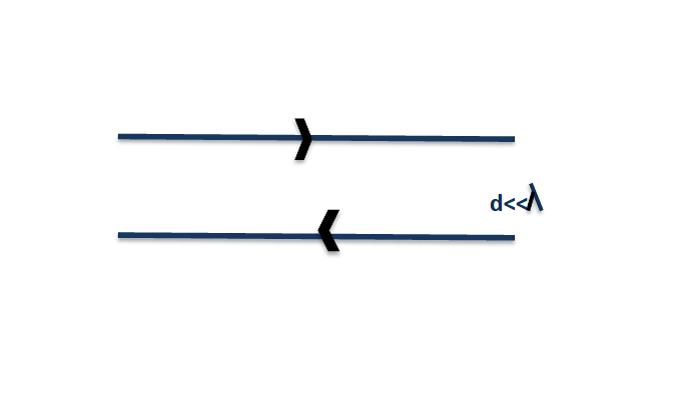
\includegraphics[width=0.8\linewidth]{\pathtoparttwo/graphics/fig_1}
\caption{Arbitrary transmission line}
\label{fig:txnsline}
\end{figure}

As discussed in the previous chapters about waveguides, such transmission lines completely guide the electromagnetic energy within their structure. This can be understood from the electric current standing wave equation given by
\begin{align*}
I(l)=\dfrac{V^+}{Z_0}e^{-\gamma l} - \dfrac{V^-}{Z_0}e^{-\gamma l}
\end{align*}
The terms of the equation show that the travelling electric currents are travelling in opposite directions as shown in figure~\ref{fig:txnsline}. Essentially the field produced by each of the time-varying components cancels out because the distance between the lines is extremely small, i.e., $d\ll\lambda$. 

So though we have accelerated and decelerated charges, we do not have radiation. However, we can say that there is a possibility of radiation because accelerated and decelerated charges are capable of giving radiation. However, if the distance between the lines in figure~\ref{fig:txnsline} is separated further such that $d\approx\lambda$, then the cancellation of fields will not take place in all directions. That is, if the field components cancel in one direction, in some other direction it is possible that the phase of the wave is changed due to the phase difference between propagating waves of the two currents and there might be radiation from the structure.
Therefore, it appears that for radiation to occur, there have two conditions that are satisfied and they are; 
\begin{enumerate}[(i)]
\item There must be time-varying currents; and
\item There must be a spatial imbalance of the currents.
\end{enumerate}
Now let's identify structures where these conditions are clearly specified.

\subsection{Radiation Phenomenon}
Now we understand the criteria for radiation, it is important to note that as frequency increases, the acceleration and deceleration of charges will increase because the rate at which the current is changing is higher. Hence as frequency increase for the same amplitude of currents, same peak current, or root-mean-square (RMS) current, we should get more radiation. Thus, in designing any antenna, we will want the structure to give radiation effectively. Also, we will want the structure to transfer a sufficient amount of power in the form of electromagnetic waves which will take the power away from the transmission line structure. Just as an illustration we take a transmission line whose characteristic impedance is known and then flare the end of the structure so that $d\approx\lambda$ such that there is the possibility of radiation (see figure~\ref{fig:flaredtxnsline}). Recall that the characteristic impedance of a transmission line depends on the inductance per unit, L, and capacitance per unit, C. For effective power transfer, we recall that the impedance of the load end (which in this case is the impedance seen by the wave as it propagates from the guided structure to space) must match the characteristic impedance $Z_0$. So if we strive to maintain maximum power transfer then the flaring of the end of the transmission line is controlled (gradual) such that the characteristic impedance at the end of the transmission line just matches the impedance seen by the wave which is $377\Omega$ for free space.

By controlling the flaring we vary L and C and thus vary $Z_0$
\begin{figure}[h]
\centering
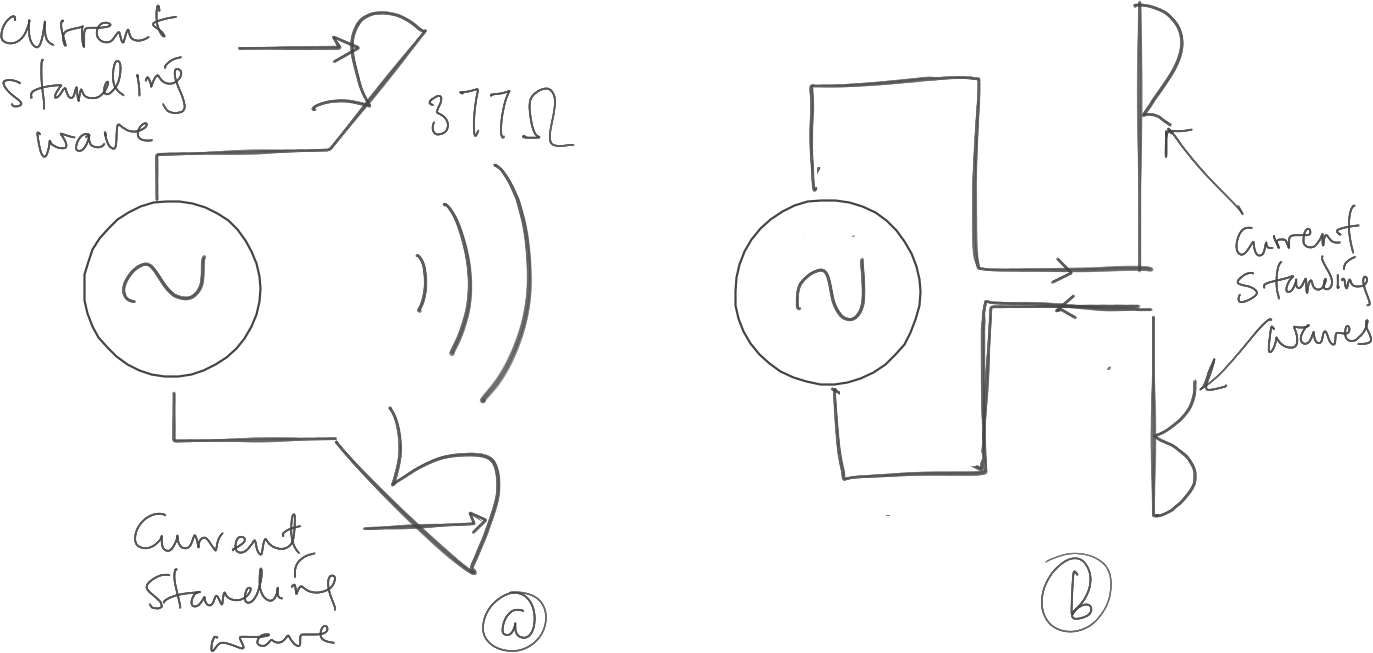
\includegraphics[width=1\linewidth]{\pathtoparttwo/graphics/txnsline}
\caption{Flared transmission line in progression showing current standing waves: (a) Flared transmission line at an angle of 60\textdegree (b) Flared transmission line at an angle of 90\textdegree}
\label{fig:flaredtxnsline}
\end{figure}

Also, we can take an extreme case and still have the nature of the standing wave retained in the transmission line when the ends are flared completely as shown in figure~\ref{fig:flaredtxnsline}(b). In this case, the current distribution is in the same direction and is generating fields that will not cancel each other.

These concepts we will discuss in some detail and give answers to questions like \emph{how much power is radiated and in which direction would the power not be radiated? What kind of polarization will be developed by the structure?} and so on.

Given the phenomenon of radiation in an antenna structure, we would say the structure has dual nature that is on one side, it acts as a circuit element with input impedance and bandwidth range, while on the other side, it generates electric and magnetic fields with characteristics that flow in a given direction and with a given power. This is illustrated in figure~\ref{fig:antennadualnature} and the characteristics of the antenna are given in table~\ref{tab:antennachar}.
\begin{figure}[h]
\centering
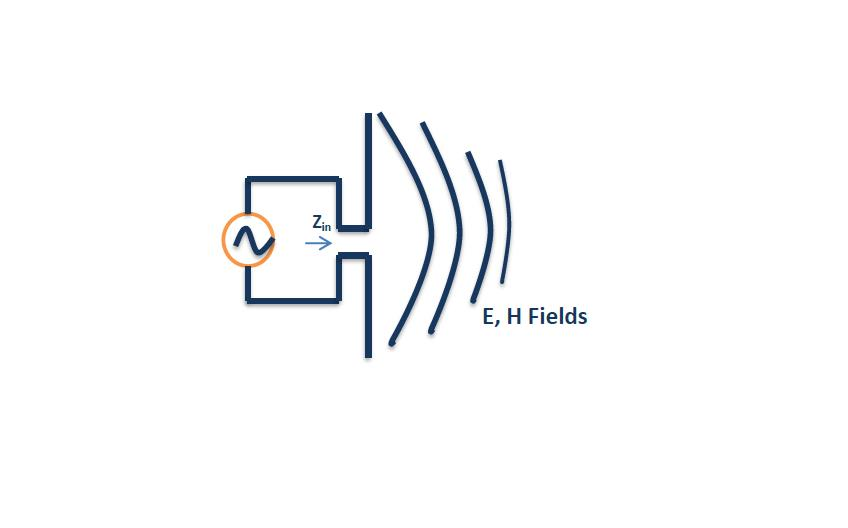
\includegraphics[width=0.8\linewidth]{\pathtoparttwo/graphics/fig_3}
\caption{Antenna structure with dual nature}
\label{fig:antennadualnature}
\end{figure}
\begin{table}[h]
\centering
\caption{Antenna characteristics}
\begin{tabular}{|l|l|}
\hline
\textbf{Circuit Characteristics} & \textbf{Wave Characteristics} \\
\hline
Input Impedance & Kind of Polarization \\
\hline
Bandwidth & Power Radiated \\
\hline
  & Directional Characteristics \\
\hline
\end{tabular}
\label{tab:antennachar}
\end{table}

Essentially, when investigating antennas, we consider the dual nature and concern ourselves with the input side when the antenna acts as a circuit element as well as treat it as a source of electromagnetic waves and provides their characteristics. 

\section{Mathematical Modeling of Radiation}
To model radiation, we refer back to Maxwell's equations. In previous chapters, when modeling electromagnetic waves we considered both a source-free medium and a medium with finite conductivity. In a medium of finite conductivity, we had conduction current density, but in this case, we would separate these two mediums when modeling radiation. One region would be the source region where there are currents and charges and there is a different region where there would be the electric and magnetic fields.
\begin{figure}[h]
\centering
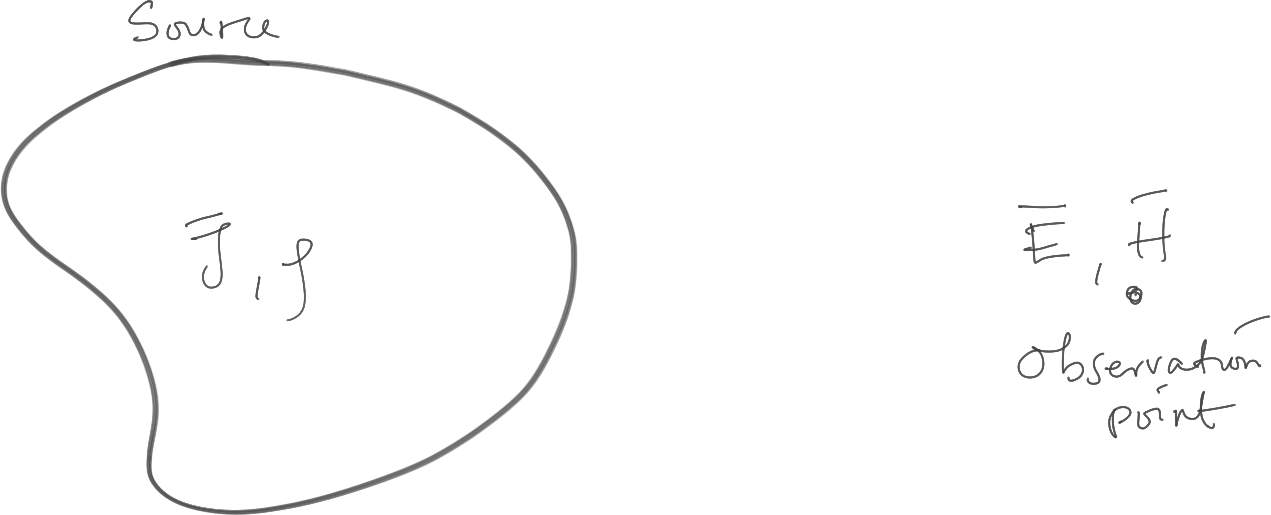
\includegraphics[width=0.8\linewidth]{\pathtoparttwo/graphics/mathematicalmodel}
\caption{Mathematical model}
\label{fig:mathematicalmodel}
\end{figure}

Let's consider a source of conduction current density $\vec{J}$ and volume charge density $\rho$ which produces electric and magnetic fields at some point called the observation point which source free as shown in figure~\ref{fig:mathematicalmodel}. The objective would be to establish the relationship between the electric and magnetic fields with the sources.

Some points to note in this analysis are;
\begin{enumerate}[(i)]
\item Previously when analyzing electromagnetic wave (the uniform plane wave) the source was pushed to infinity while here, the sources are at an observable distance from the point of reference.
\item When we analyzed the uniform plane wave we were not concerned with the choice of coordinate system to use and it was possible to model in the cartesian coordinate system which was an easier choice because the coordinates are not changing with direction but in this case, the choice of coordinate system matters and the appropriate choice is the spherical coordinate system.
\end{enumerate}

So the coordinate system normally used for antennas is the spherical coordinate system, as shown in figure~\ref{fig:sphericalcoordinate}. Again, the coordinate system is made up of the radial distance, $\rho$, the azimuthal angle, $\phi$, and the polar angle, $\theta$. The radial distance is the distance from the origin to the point of interest, the azimuthal angle is the angle measured from the x-axis in the x-y plane, and the polar angle is the angle measured from the z-axis. The unit vectors in the spherical coordinate system are $\hat{\rho}$, $\hat{\phi}$, and $\hat{\theta}$.
\begin{figure}[h]
\centering
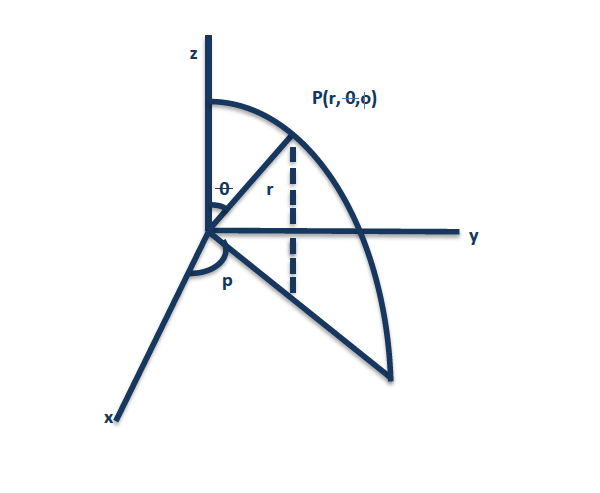
\includegraphics[width=0.8\linewidth]{\pathtoparttwo/graphics/fig_5}
\caption{Spherical coordinate}
\label{fig:sphericalcoordinate}
\end{figure}

With that established let us present Maxwell's equations as follows:
\begin{align}
\nabla\cdot\vec{D} =\rho&\text{ or }\nabla \cdot\vec{E} =\dfrac{\rho}{\epsilon}\label{eqn:gausslaw}\\
\nabla\cdot\vec{B}&=0\label{eqn:divergenceofmagneticfield}\\
\nabla\times\vec{E}&=- \dfrac{\partial\vec{B}}{\partial t}\label{eqn:faradayslaw}\\
\nabla\times\vec{H}&=\bar{J}+\dfrac{\partial\bar{D}}{\partial t}\label{eqn:ampereslaw}
\end{align}
From equation~\eqref{eqn:divergenceofmagneticfield}, $\nabla\cdot\vec{B}=0$, the condition is still satisfied if it is rewritten as $\nabla\cdot(\nabla\times\vec{A})=0$, and we call the vector $\vec{A}$ the \emph{magnetic vector potential}\index{magnetic vector potential}. Recall from the electrostatic case that calculating the electric field for any problem was best approached by finding the scalar potential and this approach is applied here such that $\vec{B}=\nabla\times\vec{A}$ which simplifies the solution.

Our objectives are as follows
\begin{enumerate}[(i)]
\item Find the solution for the potential $\vec{A}$
\item Find the magnetic and electric fields and
\item Find the power radiated from the sources
\end{enumerate}

\subsubsection*{Solution for the potential $\vec{A}$}
From equation~\eqref{eqn:faradayslaw}
\begin{align*}
&\nabla\times\vec{E}=\dfrac{-\partial(\nabla\times\vec{A})}{\partial t}&\\
&\text{Interchanging the time and space derivatives gives}&\\
&\nabla\times\vec{E}=-\nabla\times\dfrac{-\partial\vec{A}}{\partial t}&\\
&\text{Let represent a time derivative with a dot }(\cdot)\text{ on the vector}&\\
&\nabla\times\vec{E}=-\nabla\times\dot{\vec{A}}&\\
&\nabla\times(\vec{E}+\dot{\vec{A}})=0&\\
&\text{Still the expression can be written as}&\\
&\vec{E}+\dot{\vec{A}}= -\nabla V\quad\text{since }\nabla\times(-\nabla V)=0&
\end{align*}
The minus sign is placed to retain the relationship between $\vec{E}$ and $V$. If the time-varying magnetic scalar vector $\dot{\vec{A}}$ is removed from the expression.

From equation~\eqref{eqn:ampereslaw}, $\nabla\times\vec{H}=\vec{J}+\dot{\vec{D}}$
and $\vec{D}=\epsilon\vec{E}$. Then,
\begin{align}
\nabla\times\vec{H}=\vec{J}+\epsilon\dot{\vec{E}}\footnotemark
\label{eqn:ampereslawwithepsilon}
\end{align}
\footnotetext{
We assume $\epsilon$ is not a function of time - a homogeneous medium
}
From $\vec{B}=\nabla\times\vec{A}$ and $\vec{B}=\mu\vec{H}$, then
\begin{align*}
\mu\vec{H}=\nabla\times\vec{A}
\end{align*}
\begin{equation}
\vec{H}=\dfrac{1}{\mu}\nabla\times\vec{A}
\label{eqn:magneticfieldtovectorpotential}
\end{equation}
Substitute equation~\eqref{eqn:magneticfieldtovectorpotential} in~\eqref{eqn:ampereslawwithepsilon} gives
\begin{align*}
&\nabla\times\left(\dfrac{1}{\mu}\nabla\times\vec{A}\right)=\vec{J}+\epsilon\dot{\vec{E}}\footnotemark&\\
&\nabla\times\nabla\times\vec{A}=\mu\vec{J}+\mu\epsilon\dot{\vec{E}}&\\
&\text{Using vector identities}&\\
&\nabla\times\nabla\times\vec{A}=\nabla(\nabla\cdot\vec{A}) -\nabla^{2}\vec{A}=\mu\vec{J}+\mu\epsilon\dot{\vec{E}}&\\
&\text{Substituting $\dot{\vec{E}}=-(\nabla\dot{V}+\ddot{\vec{A}})$}&\\
&\nabla(\nabla\cdot\vec{A}) -\nabla^{2}\vec{A}=\mu\vec{J}+\mu\epsilon(-(\nabla\dot{V}+\ddot{\vec{A}}))&\\
&\nabla(\nabla\cdot\vec{A}) -\nabla^{2}\vec{A}=\mu\vec{J}+\mu\epsilon\nabla\dot{V}-\mu\epsilon\vec{A}&
\end{align*}
\footnotetext{
Also, $\mu$ is not a function of space (isotropic)
}
Rewriting the expression
\begin{equation}
\nabla^{2}\vec{A}-\mu\epsilon\ddot{\vec{A}}=-\mu\vec{J}+\mu\epsilon\nabla\dot{V}+\nabla(\nabla\cdot\vec{A})
\label{eqn:vectorpotentialeqn}
\end{equation}
When the equation~\ref{eqn:vectorpotentialeqn} is compared with the equation of electric and magnetic fields in a source-free unbound medium (if we set $\vec{J}$ to zero for $\sigma=0$). It is seen that the above equation has the components $\mu\epsilon\nabla\dot{V}$ and $\nabla(\nabla\cdot\vec{A})$, in addition, compare to the equations of the electric and magnetic fields in a source-free unbounded medium which are given by
\begin{align*}
\nabla^{2}\vec{E}-\mu\epsilon\ddot{\vec{E}}=0\\
\nabla^{2}\vec{H}-\mu\epsilon\ddot{\vec{H}}=0
\end{align*}

If these solutions satisfy the same boundary conditions\textemdash it is source-free and an unbound medium\textemdash then from the \emph{uniqueness theorem}\index{uniqueness theorem}, they are indeed the same solution. Hence we can make equation~\eqref{eqn:vectorpotentialeqn} unique by satisfying the uniqueness theorem and defining the expression for the divergence of the vector $A$.

Hence,
\begin{align*}
\mu\epsilon\nabla\dot{V}+\nabla(\nabla\cdot\vec{A})&=0\\
\nabla(\mu\epsilon\dot{V}+\nabla\cdot\vec{A})&=0
\end{align*}
Then,
\begin{align}
\nabla\cdot\vec{A}=-\mu\epsilon\dot{V}
\label{eqn:lorentzguagecondition}
\end{align}
Equation~\eqref{eqn:lorentzguagecondition} is called the \emph{Lorentz gauge condition}\index{lorentz gauge condition}. This condition defines the divergence of the magnetic vector potential
Now equation~\eqref{eqn:vectorpotentialeqn} reduces to
\begin{equation}
\nabla^{2}\vec{A}-\mu\epsilon\ddot{\vec{A}}=-\mu\vec{J}
\label{eqn:vectorpotentialeqnwithlorentzguage}
\end{equation} 
Take the divergence of $\vec{E}+\dot{\vec{A}}=-\mu\vec{J}$ to give;
\begin{align*}
&\nabla\cdot\vec{E}+\nabla\cdot\dot{\vec{A}}=-\nabla^{2} V&\\
&\text{Substituting $\nabla\cdotp\dot{\vec{A}}=-\mu\epsilon\ddot{V}$}&\\
&\nabla\cdotp\vec{E}-\mu\epsilon\ddot{V}=-\nabla^{2} V&\\
&\text{Rearranging}&\\
&\nabla^{2} V-\mu\epsilon\ddot{V}=-\nabla\cdotp\vec{E}&\\
&\text{From $\nabla\cdotp\vec{E}=\dfrac{\rho}{\epsilon}$, We get}&
\end{align*}
\begin{equation}
\nabla\dot\vec{E}-\mu\epsilon\ddot{V}=-\dfrac{\rho}{\epsilon}
\label{eqn:scalarpotential}
\end{equation}

Both equations~\eqref{eqn:vectorpotentialeqnwithlorentzguage} and~\eqref{eqn:scalarpotential} can be rewritten as
\begin{align*}
\Box\vec{A}=\mu J\\
\Box V=\dfrac{\rho}{\epsilon}\\
\end{align*}
Where $\Box$ is called the D'Alembertian Operator or box operator given by 
\begin{align*}
\Box=\dfrac{\partial^{2}}{\partial t^{2}}-\dfrac{1}{c^{2}}\nabla^{2}
\end{align*}
With the Lorentz gauge condition, we get an identical solution to equation~\eqref{eqn:vectorpotentialeqnwithlorentzguage} for the scalar potential $V$. This expression shows that the magnetic vector potential is related to the conduction current density, $\vec{J}$, and the scalar potential is related to the volume charge density, $\rho$.

In conclusion, when we have time-varying sources, we would have electric potential and magnetic vector potential and both are essentially governed by the wave equation; which implies they have wave behaviour in the 3-dimensional space.
